\documentclass{article}
%%%%%%%%%%%%%
% Loads packages
%%%%%%%%%%%%%
\usepackage[table]{xcolor}
\usepackage[utf8]{inputenc}
\usepackage[colorlinks=true,linkcolor=blue]{hyperref}
\usepackage{geometry} %package needed to set margins
\usepackage{fancyhdr}
\usepackage{graphicx}
\usepackage{amsmath}
\usepackage{amsthm}
\usepackage{mdframed}
\usepackage{tikz}
\usetikzlibrary{arrows.meta}
\usetikzlibrary{decorations.markings}
\usepackage{amsfonts}
\usepackage{wasysym}
\usepackage{listings}% http://ctan.org/pkg/listings
\lstset{
basicstyle=\ttfamily,
mathescape
}
\pagestyle{fancy}
\fancyhf{}
\chead{\textbf{Homework 10}}
\lhead{Math 213, Fall 2024}
\rhead{Due Sunday, 11/17 at 11:59pm}
%%%%%%%%%%%%%
% Sets margins
%%%%%%%%%%%%%
\newgeometry{left=1.5in,right=1in,top=1in,bottom=1in}
\setlength\headsep{3pt}
%%%%%%%%%%%%%
% Creates problem and solution environments
%%%%%%%%%%%%%
% Solution Environment
\newenvironment{solution}{\begin{proof}[Solution]}{\end{proof}}
% Problem Environment
\newenvironment{problem}[1]
{\begin{mdframed}[default]
\textbf{Problem #1:}
}
{\end{mdframed}
}
%%%%%%%%%%%
% Custom Commands
%%%%%%%%%%%
\newcommand{\gOne}{\cellcolor{green!50!white} 1}
\newcommand{\rZero}{\cellcolor{red!50!white} 0}
\begin{document}
\begin{problem}{\S 10.3 - 14}
Represent the following graph using an adjacency matrix.
\begin{center}
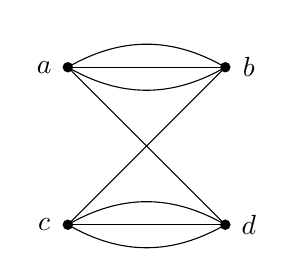
\begin{tikzpicture}
% draws vertices
\node[circle, fill=black,scale = 0.4] at (0,0){};
\node[circle, fill=black,scale = 0.4] at (0,2){};
\node[circle, fill=black,scale = 0.4] at (2,0){};
\node[circle, fill=black,scale = 0.4] at (2,2){};
% draws edges
\draw (0,0) to (2,2);
\draw (0,2) to (2,0);
\draw (0,0) to (2,0);
\draw[out=30,in=150] (0,0) to (2,0);
\draw[out=-30,in=-150] (0,0) to (2,0);
\draw (0,2) to (2,2);
\draw[out=30,in=150] (0,2) to (2,2);
\draw[out=-30,in=-150] (0,2) to (2,2);
% labels vertices
\node at (-0.3,2) {$a$};
\node at (2.3,2) {$b$};
\node at (-0.3,0) {$c$};
\node at (2.3,0) {$d$};
\end{tikzpicture}
\end{center}
Solution:

\[\begin{bmatrix} 0 & 3 & 0 & 1 \\ 3 & 0 & 1 & 0 \\ 0&1&0&3 \\ 1&0&3&0 \end{bmatrix}\]
\end{problem}
\begin{problem}{\S 10.3 - 20}
Find the adjacency matrix of the given directed multigraph with respect to the
vertices listed in alphabetic order.
\begin{center}
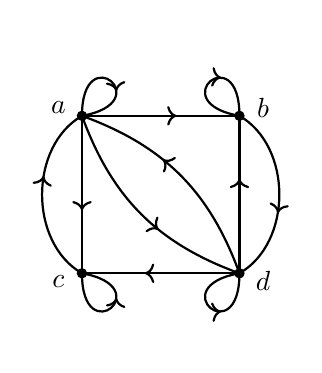
\begin{tikzpicture}
\begin{scope}[thick,decoration={
markings,
mark=at position 0.6 with {\arrow{>}}}
]
% draws vertices
\node[circle, fill=black,scale = 0.4] at (0,0){};
\node[circle, fill=black,scale = 0.4] at (0,2){};
\node[circle, fill=black,scale = 0.4] at (2,0){};
\node[circle, fill=black,scale = 0.4] at (2,2){};
% draws edges
\draw[postaction={decorate}] (2,0) to (0,0);
\draw[postaction={decorate}] (0,2) to (2,2);
\draw[postaction={decorate},out=150,in=-150] (0,0) to (0,2);
\draw[postaction={decorate}] (0,2) to (0,0);
\draw[postaction={decorate}] (2,0) to (2,2);
\draw[postaction={decorate},out=-30,in=30] (2,2) to (2,0);
\draw[postaction={decorate},out=-70,in=160] (0,2) to (2,0);
\draw[postaction={decorate},out=110,in=-20] (2,0) to (0,2);
% draw loops
\draw[scale=2,postaction={decorate}] (1,0) to[out=-170, in=-90,loop]
(1,0);
\draw[scale=2,postaction={decorate}] (0,0) to[out=-90, in=-10,loop]
(0,0);
\draw[scale=2,postaction={decorate}] (1,1) to[out=170, in=90,loop]
(1,1);
\draw[scale=2,postaction={decorate}] (0,1) to[out=90, in=10,loop]
(0,1);
% labels vertices
\node at (-0.3,2.1) {$a$};
\node at (2.3,2.1) {$b$};
\node at (-0.3,-0.1) {$c$};
\node at (2.3,-0.1) {$d$};
\end{scope}
\end{tikzpicture}
\end{center}
Solution:
\[\begin{bmatrix} 1&1&1&1 \\ 0&1&0&1 \\ 1&0&1&0 \\ 1&1&1&1 \end{bmatrix}\]
\end{problem}
\begin{problem}{\S 10.3 - 26}
Use incidence matrices to represent the following graphs:
\begin{center}
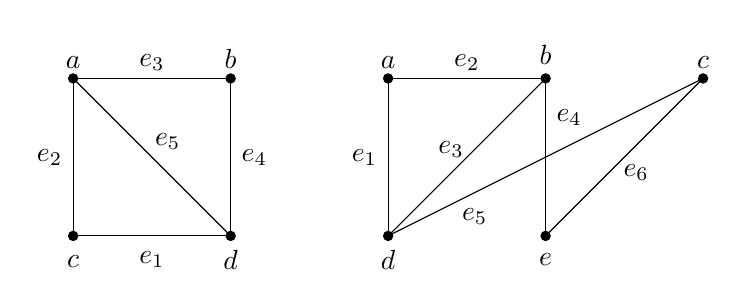
\begin{tikzpicture}
%%% Draws graph 1
% draws vertices
\node[circle, fill=black,scale = 0.4] at (0,0){};
\node[circle, fill=black,scale = 0.4] at (0,2){};
\node[circle, fill=black,scale = 0.4] at (2,0){};
\node[circle, fill=black,scale = 0.4] at (2,2){};
% draws edges
\draw (0,0) to (2,0) to (2,2) to (0,2) to (0,0);
\draw (0,2) to (2,0);
% labels vertices
\node at (0,2.2) {$a$};
\node at (2,2.25) {$b$};
\node at (0,-0.32) {$c$};
\node at (2,-0.3) {$d$};
% labels edges
\node at (1,-0.3) {$e_1$};
\node at (-0.3,1) {$e_2$};
\node at (1,2.2) {$e_3$};
\node at (2.3,1) {$e_4$};
\node at (1.2,1.2) {$e_5$};
%%% Draws graph 2
% draws vertices
\node[circle, fill=black,scale = 0.4] at (4,0){};
\node[circle, fill=black,scale = 0.4] at (6,0){};
\node[circle, fill=black,scale = 0.4] at (4,2){};
\node[circle, fill=black,scale = 0.4] at (6,2){};
\node[circle, fill=black,scale = 0.4] at (8,2){};
% draws edges
\draw (4,0) to (4,2) to (6,2) to (6,0);
\draw (6,2) to (4,0) to (8,2) to (6,0);
% label vertices
\node at (4,2.2) {$a$};
\node at (6,2.3) {$b$};
\node at (8,2.2) {$c$};
\node at (4,-0.3) {$d$};
\node at (6,-0.3) {$e$};
% label edges
\node at (3.7,1) {$e_1$};
\node at (5,2.2) {$e_2$};
\node at (4.8,1.1) {$e_3$};
\node at (6.3,1.5) {$e_4$};
\node at (5.1,0.25) {$e_5$};
\node at (7.15,0.8) {$e_6$};
\end{tikzpicture}
\end{center}
Solution:
For left graph:
\[\begin{bmatrix}
    0&1&1&0&1 \\
    0&0&1&1&0 \\
    1&1&0&0&0 \\
    1&0&0&1&1 \\
\end{bmatrix}\]
For right graph:
\[\begin{bmatrix}
    1&1&0&0&0&0 \\
    0&1&1&1&0&0 \\
    0&0&0&0&1&1 \\
    1&0&1&0&1&0 \\
    0&0&0&1&0&1 \\
\end{bmatrix}\]
\end{problem}
\begin{problem}{\S 10.3 - 34}
Determine if the given pair of graphs is isomorphic. Either exhibit an isomorphism
or provide a rigorous argument that none exists.
\begin{center}
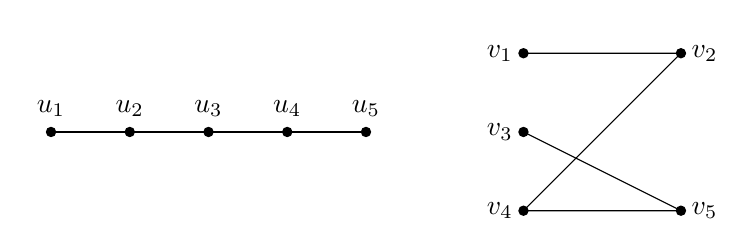
\begin{tikzpicture}
%%% Draws left graph
% draws vertices
\node[circle, fill=black,scale = 0.4] at (0,0){};
\node[circle, fill=black,scale = 0.4] at (1,0){};
\node[circle, fill=black,scale = 0.4] at (2,0){};
\node[circle, fill=black,scale = 0.4] at (3,0){};
\node[circle, fill=black,scale = 0.4] at (4,0){};
% draws edges
\draw (0,0) to (4,0);
% label vertices
\node at (0,0.3) {$u_1$};
\node at (1,0.3) {$u_2$};
\node at (2,0.3) {$u_3$};
\node at (3,0.3) {$u_4$};
\node at (4,0.3) {$u_5$};
%%% Draws right graph
% draws vertices
\node[circle, fill=black,scale = 0.4] at (6,0){};
\node[circle, fill=black,scale = 0.4] at (6,-1){};
\node[circle, fill=black,scale = 0.4] at (6,1){};
\node[circle, fill=black,scale = 0.4] at (8,1){};
\node[circle, fill=black,scale = 0.4] at (8,-1){};
% draws edges
\draw (6,0) to (8,-1) to (6,-1) to (8,1) to (6,1);
% labels vertices
\node at (5.7,-1) {$v_4$};
\node at (8.3,-1) {$v_5$};
\node at (5.7,0) {$v_3$};
\node at (5.7,1) {$v_1$};
\node at (8.3,1) {$v_2$};
\end{tikzpicture}
\end{center}
Solution:

It is isomorphic, there are 5 vertices, 4 edges for both graphs, the degree sequence for both graph is $[1,2,2,2,1]$ and $[1,2,2,2,1]$, there exist an bijection function from left to right graph: $f(u_1)=v_1$, $f(u_2)=v_2$, $f(u_3)=v_4$, $f(u_4)=v_5$, $f(u_5)=v_3$.
\end{problem}
\begin{problem}{\S 10.3 - 36}
Determine if the given pair of graphs is isomorphic. Either exhibit an isomorphism
or provide a rigorous argument that none exists.
\begin{center}
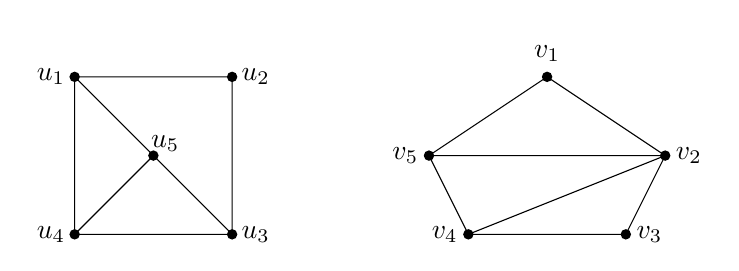
\begin{tikzpicture}
%%% Draws left graph
% draws vertices
\node[circle, fill=black,scale = 0.4] at (0,0){};
\node[circle, fill=black,scale = 0.4] at (2,0){};
\node[circle, fill=black,scale = 0.4] at (0,2){};
\node[circle, fill=black,scale = 0.4] at (2,2){};
\node[circle, fill=black,scale = 0.4] at (1,1){};
% draws edges
\draw (0,0) to (2,0) to (2,2) to (0,2) to (0,0) to (1,1) to (2,0);
\draw (0,2) to (1,1);
% labels vertices
\node at (-0.3,0) {$u_4$};
\node at (-0.3,2) {$u_1$};
\node at (2.3,0) {$u_3$};
\node at (2.3,2) {$u_2$};
\node at (1.15,1.15) {$u_5$};
%%% Draws right graph
% draws vertices
\node[circle, fill=black,scale = 0.4] at (5,0){};
\node[circle, fill=black,scale = 0.4] at (7,0){};
\node[circle, fill=black,scale = 0.4] at (6,2){};
\node[circle, fill=black,scale = 0.4] at (4.5,1){};
\node[circle, fill=black,scale = 0.4] at (7.5,1){};
% draws edges
\draw (5,0) to (7,0) to (7.5,1) to (6,2) to (4.5,1) to (5,0) to (7.5,1) to
(4.5,1);
% labels vertices
\node at (4.7,0) {$v_4$};
\node at (4.2,1) {$v_5$};
\node at (6,2.3) {$v_1$};
\node at (7.8,1) {$v_2$};
\node at (7.3,0) {$v_3$};
\end{tikzpicture}
\end{center}
Solution:

there are 5 vertices, 7 edges for both graphs, the degree sequence of left graph is $[3,2,3,3,3]$, right graph: $[2,4,2,3,3]$, the degree sequence is different, so it is not isomorphic.
\end{problem}
\begin{problem}{\S 10.3 - 40}
Determine if the given pair of graphs is isomorphic. Either exhibit an isomorphism
or provide a rigorous argument that none exists.
\begin{center}
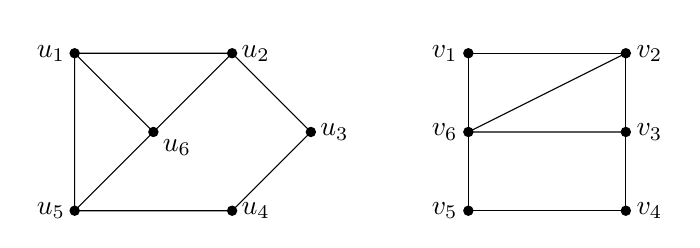
\begin{tikzpicture}
%%% Draws left graph
% draws vertices
\node[circle, fill=black,scale = 0.4] at (0,0){};
\node[circle, fill=black,scale = 0.4] at (2,0){};
\node[circle, fill=black,scale = 0.4] at (1,1){};
\node[circle, fill=black,scale = 0.4] at (3,1){};
\node[circle, fill=black,scale = 0.4] at (0,2){};
\node[circle, fill=black,scale = 0.4] at (2,2){};
% draws edges
\draw (0,0) to (2,0) to (3,1) to (2,2) to (0,2) to (0,0) to (1,1) to (2,2);
\draw (1,1) to (0,2);
% labels vertices
\node at (-0.3,0) {$u_5$};
\node at (-0.3,2) {$u_1$};
\node at (2.3,2) {$u_2$};
\node at (3.3,1) {$u_3$};
\node at (1.3,0.8) {$u_6$};
\node at (2.3,0) {$u_4$};
%%% Draws right graph
% draws vertices
\node[circle, fill=black,scale = 0.4] at (5,0){};
\node[circle, fill=black,scale = 0.4] at (7,0){};
\node[circle, fill=black,scale = 0.4] at (5,1){};
\node[circle, fill=black,scale = 0.4] at (7,1){};
\node[circle, fill=black,scale = 0.4] at (5,2){};
\node[circle, fill=black,scale = 0.4] at (7,2){};
% draws edges
\draw (5,0) to (7,0) to (7,2) to (5,2) to (5,0);
\draw (7,1) to (5,1) to (7,2);
% labels vertices
\node at (4.7,0) {$v_5$};
\node at (7.3,0) {$v_4$};
\node at (7.3,1) {$v_3$};
\node at (7.3,2) {$v_2$};
\node at (4.7,1) {$v_6$};
\node at (4.7,2) {$v_1$};
\end{tikzpicture}
\end{center}
Solution:

There are 6 vertices for both graph, and 8 edges for both graph. The degree sequence for left graph is $[3,3,2,2,3,3]$, for right graph is $[2,3,3,2,2,4]$, the degree sequence is different, so it is not isomorphic.
\end{problem}
\begin{problem}{\S 10.4 - 12}
Determine whether each of these graphs is strongly connected and if not, whether it
is weakly connected.
\begin{enumerate}
\item[(a)] \;
\begin{center}
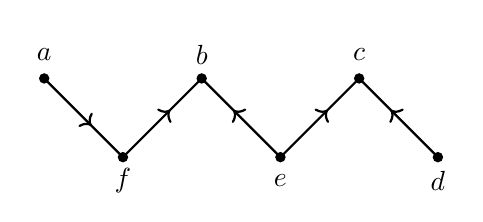
\begin{tikzpicture}
\begin{scope}[thick,decoration={
markings,
mark=at position 0.6 with {\arrow{>}}}
]
% draws vertices
\node[circle, fill=black,scale = 0.4] at (0,1){};
\node[circle, fill=black,scale = 0.4] at (1,0){};
\node[circle, fill=black,scale = 0.4] at (2,1){};
\node[circle, fill=black,scale = 0.4] at (3,0){};
\node[circle, fill=black,scale = 0.4] at (4,1){};
\node[circle, fill=black,scale = 0.4] at (5,0){};
% labels vertices
\node at (0,1.3) {$a$};
\node at (1,-0.3) {$f$};
\node at (2,1.3) {$b$};
\node at (3,-0.3) {$e$};
\node at (4,1.3) {$c$};
\node at (5,-0.3) {$d$};
% draws edges
\draw[postaction={decorate}] (0,1) to (1,0);
\draw[postaction={decorate}] (1,0) to (2,1);
\draw[postaction={decorate}] (3,0) to (2,1);
\draw[postaction={decorate}] (3,0) to (4,1);
\draw[postaction={decorate}] (5,0) to (4,1);
\end{scope}
\end{tikzpicture}
\end{center}
\item[(b)] \;
\begin{center}
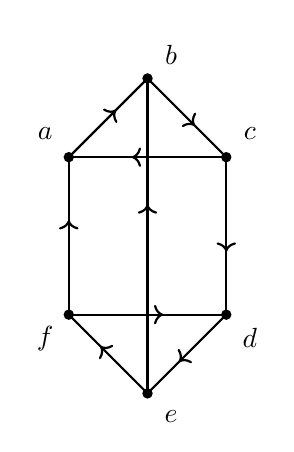
\begin{tikzpicture}
\begin{scope}[thick,decoration={
markings,
mark=at position 0.6 with {\arrow{>}}}
]
% draws vertices
\node[circle, fill=black,scale = 0.4] at (-1,1){};
\node[circle, fill=black,scale = 0.4] at (0,2){};
\node[circle, fill=black,scale = 0.4] at (1,1){};
\node[circle, fill=black,scale = 0.4] at (1,-1){};
\node[circle, fill=black,scale = 0.4] at (0,-2){};
\node[circle, fill=black,scale = 0.4] at (-1,-1){};
% labels vertices
\node at (-1.3,1.3) {$a$};
\node at (0.3,2.3) {$b$};
\node at (1.3,1.3) {$c$};
\node at (1.3,-1.3) {$d$};
\node at (0.3,-2.3) {$e$};
\node at (-1.3,-1.3) {$f$};
% draws edges
\draw[postaction={decorate}] (-1,1) to (0,2);
\draw[postaction={decorate}] (0,2) to (1,1);
\draw[postaction={decorate}] (1,1) to (1,-1);
\draw[postaction={decorate}] (1,-1) to (0,-2);
\draw[postaction={decorate}] (0,-2) to (-1,-1);
\draw[postaction={decorate}] (-1,-1) to (-1,1);
\draw[postaction={decorate}] (1,1) to (-1,1);
\draw[postaction={decorate}] (-1,-1) to (1,-1);
\draw[postaction={decorate}] (0,-2) to (0,2);
\end{scope}
\end{tikzpicture}
\end{center}
\item[(c)] \;
\begin{center}
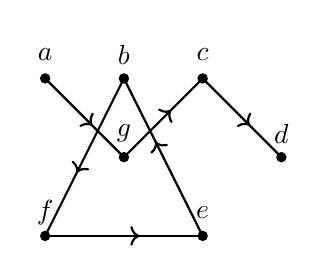
\begin{tikzpicture}
\coordinate (a) at (0,2);
\coordinate (b) at (1,2);
\coordinate (c) at (2,2);
\coordinate (d) at (3,1);
\coordinate (e) at (2,0);
\coordinate (f) at (0,0);
\coordinate (g) at (1,1);
\begin{scope}[thick,decoration={
markings,
mark=at position 0.6 with {\arrow{>}}}
]
% draws vertices
\node[circle, fill=black,scale = 0.4] at (a){};
\node[circle, fill=black,scale = 0.4] at (b){};
\node[circle, fill=black,scale = 0.4] at (c){};
\node[circle, fill=black,scale = 0.4] at (d){};
\node[circle, fill=black,scale = 0.4] at (e){};
\node[circle, fill=black,scale = 0.4] at (f){};
\node[circle, fill=black,scale = 0.4] at (g){};
% labels vertices
\node at (0,2.3) {$a$};
\node at (1,2.3) {$b$};
\node at (2,2.3) {$c$};
\node at (3,1.3) {$d$};
\node at (2,0.3) {$e$};
\node at (0,0.3) {$f$};
\node at (1,1.3) {$g$};
% draws edges
\draw[postaction={decorate}] (a) to (g);
\draw[postaction={decorate}] (g) to (c);
\draw[postaction={decorate}] (c) to (d);
\draw[postaction={decorate}] (b) to (f);
\draw[postaction={decorate}] (f) to (e);
\draw[postaction={decorate}] (e) to (b);
\end{scope}
\end{tikzpicture}
\end{center}
\end{enumerate}
Solution:
\begin{enumerate}
    \item[(a)] All vertices are connected, so it is connected, but there don't exist path in this directed graph from any vertices from a to b and b to a, so it is weakly connected.
    \item[(b)] All vertices are connected by path, and for each two vertices, there exist path from a to b and b to a, so it is strongly connected.
    \item[(c)] These vertices are not connected with two group, one is $\{a,g,c,d\}$ and $\{b,f,e\}$, so, in-connected.
\end{enumerate}
\end{problem}
\begin{problem}{\S 10.4 - 20} Use paths either to show that these graphs are not
isomorphic or to find an isomorphism between these graphs.
\begin{center}
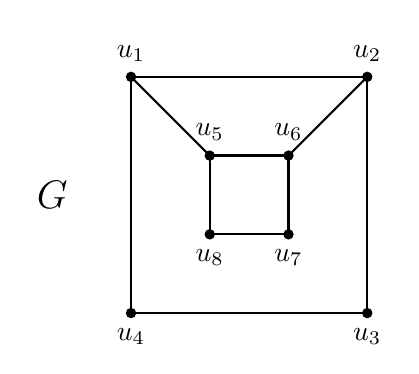
\begin{tikzpicture}
\coordinate (a) at (0,3);
\coordinate (b) at (3,3);
\coordinate (c) at (3,0);
\coordinate (d) at (0,0);
\coordinate (e) at (1,2);
\coordinate (f) at (2,2);
\coordinate (g) at (2,1);
\coordinate (h) at (1,1);
\begin{scope}[thick]
% draws vertices
\node[circle, fill=black,scale = 0.4] at (a){};
\node[circle, fill=black,scale = 0.4] at (b){};
\node[circle, fill=black,scale = 0.4] at (c){};
\node[circle, fill=black,scale = 0.4] at (d){};
\node[circle, fill=black,scale = 0.4] at (e){};
\node[circle, fill=black,scale = 0.4] at (f){};
\node[circle, fill=black,scale = 0.4] at (g){};
\node[circle, fill=black,scale = 0.4] at (h){};
% labels vertices
\node at (0,3.3) {$u_1$};
\node at (3,3.3) {$u_2$};
\node at (3,-0.3) {$u_3$};
\node at (0,-0.3) {$u_4$};
\node at (1,2.3) {$u_5$};
\node at (2,2.3) {$u_6$};
\node at (2,0.7) {$u_7$};
\node at (1,0.7) {$u_8$};
\node at (-1,1.5) {\Large $G$};
% draws edges
\draw[postaction={decorate}] (a) to (b);
\draw[postaction={decorate}] (b) to (c);
\draw[postaction={decorate}] (c) to (d);
\draw[postaction={decorate}] (d) to (a);
\draw[postaction={decorate}] (e) to (f);
\draw[postaction={decorate}] (f) to (g);
\draw[postaction={decorate}] (g) to (h);
\draw[postaction={decorate}] (h) to (e);
\draw[postaction={decorate}] (a) to (e);
\draw[postaction={decorate}] (b) to (f);
\end{scope}
\end{tikzpicture}
\end{center}
\begin{center}
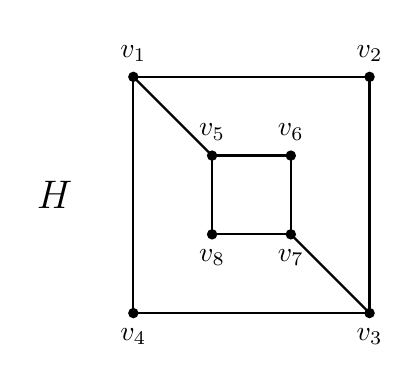
\begin{tikzpicture}
\coordinate (a) at (0,3);
\coordinate (b) at (3,3);
\coordinate (c) at (3,0);
\coordinate (d) at (0,0);
\coordinate (e) at (1,2);
\coordinate (f) at (2,2);
\coordinate (g) at (2,1);
\coordinate (h) at (1,1);
\begin{scope}[thick]
% draws vertices
\node[circle, fill=black,scale = 0.4] at (a){};
\node[circle, fill=black,scale = 0.4] at (b){};
\node[circle, fill=black,scale = 0.4] at (c){};
\node[circle, fill=black,scale = 0.4] at (d){};
\node[circle, fill=black,scale = 0.4] at (e){};
\node[circle, fill=black,scale = 0.4] at (f){};
\node[circle, fill=black,scale = 0.4] at (g){};
\node[circle, fill=black,scale = 0.4] at (h){};
% labels vertices
\node at (0,3.3) {$v_1$};
\node at (3,3.3) {$v_2$};
\node at (3,-0.3) {$v_3$};
\node at (0,-0.3) {$v_4$};
\node at (1,2.3) {$v_5$};
\node at (2,2.3) {$v_6$};
\node at (2,0.7) {$v_7$};
\node at (1,0.7) {$v_8$};
\node at (-1,1.5) {\Large $H$};
% draws edges
\draw[postaction={decorate}] (a) to (b);
\draw[postaction={decorate}] (b) to (c);
\draw[postaction={decorate}] (c) to (d);
\draw[postaction={decorate}] (d) to (a);
\draw[postaction={decorate}] (e) to (f);
\draw[postaction={decorate}] (f) to (g);
\draw[postaction={decorate}] (g) to (h);
\draw[postaction={decorate}] (h) to (e);
\draw[postaction={decorate}] (a) to (e);
\draw[postaction={decorate}] (c) to (g);
\end{scope}
\end{tikzpicture}
\end{center}
Solution:

These two graph is not isomorphic, because the second graph does not exist two 3-degree vertices that is connected, but the first have. So, they are not isomorphic.
\end{problem}
\begin{problem}{\S 10.4 - 32} Find all the cut vertices of the given graph.
\begin{center}
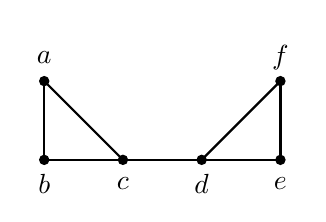
\begin{tikzpicture}
\coordinate (a) at (0,1);
\coordinate (b) at (0,0);
\coordinate (c) at (1,0);
\coordinate (d) at (2,0);
\coordinate (e) at (3,0);
\coordinate (f) at (3,1);
\begin{scope}[thick]
% draws vertices
\node[circle, fill=black,scale = 0.4] at (a){};
\node[circle, fill=black,scale = 0.4] at (b){};
\node[circle, fill=black,scale = 0.4] at (c){};
\node[circle, fill=black,scale = 0.4] at (d){};
\node[circle, fill=black,scale = 0.4] at (e){};
\node[circle, fill=black,scale = 0.4] at (f){};
% labels vertices
\node at (0,1.3) {$a$};
\node at (0,-0.3) {$b$};
\node at (1,-0.3) {$c$};
\node at (2,-0.3) {$d$};
\node at (3,-0.3) {$e$};
\node at (3,1.3) {$f$};
% draws edges
\draw[postaction={decorate}] (a) to (b);
\draw[postaction={decorate}] (b) to (c);
\draw[postaction={decorate}] (c) to (a);
\draw[postaction={decorate}] (c) to (d);
\draw[postaction={decorate}] (d) to (e);
\draw[postaction={decorate}] (e) to (f);
\draw[postaction={decorate}] (f) to (d); \end{scope}
\end{tikzpicture}
\end{center}
Solution:
vertex $c$ and $d$ are cut vertex, since remove any of them will disconnect this graph.
\end{problem}
\begin{problem}{\S 10.4 - 34} Find all the cut edges of the given graph.

\begin{center}
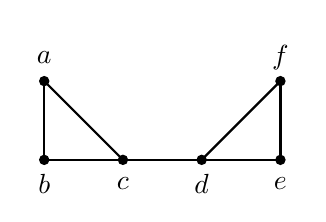
\begin{tikzpicture}
\coordinate (a) at (0,1);
\coordinate (b) at (0,0);
\coordinate (c) at (1,0);
\coordinate (d) at (2,0);
\coordinate (e) at (3,0);
\coordinate (f) at (3,1);
\begin{scope}[thick]
% draws vertices
\node[circle, fill=black,scale = 0.4] at (a){};
\node[circle, fill=black,scale = 0.4] at (b){};
\node[circle, fill=black,scale = 0.4] at (c){};
\node[circle, fill=black,scale = 0.4] at (d){};
\node[circle, fill=black,scale = 0.4] at (e){};
\node[circle, fill=black,scale = 0.4] at (f){};
% labels vertices
\node at (0,1.3) {$a$};
\node at (0,-0.3) {$b$};
\node at (1,-0.3) {$c$};
\node at (2,-0.3) {$d$};
\node at (3,-0.3) {$e$};
\node at (3,1.3) {$f$};
% draws edges
\draw[postaction={decorate}] (a) to (b);
\draw[postaction={decorate}] (b) to (c);
\draw[postaction={decorate}] (c) to (a);
\draw[postaction={decorate}] (c) to (d);
\draw[postaction={decorate}] (d) to (e);
\draw[postaction={decorate}] (e) to (f);
\draw[postaction={decorate}] (f) to (d); \end{scope}
\end{tikzpicture}
\end{center}
Solution: the edge $c-d$ is the cut edge of this graph, since remove it will disconnect this graph.
\end{problem}
\begin{problem}{\S 10.5 - 2} Determine whether the given graph has an
Euler circuit. Construct such a circuit when one exists. If
no Euler circuit exists, determine whether the graph has an
Euler path and construct such a path if one exists.
\begin{center}
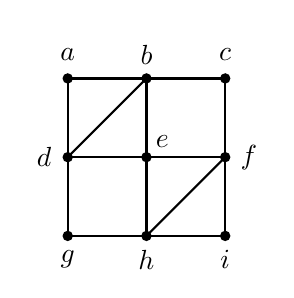
\begin{tikzpicture}
\coordinate (a) at (0,2);
\coordinate (b) at (1,2);
\coordinate (c) at (2,2);
\coordinate (d) at (0,1);
\coordinate (e) at (1,1);
\coordinate (f) at (2,1);
\coordinate (g) at (0,0);
\coordinate (h) at (1,0);
\coordinate (i) at (2,0);
\begin{scope}[thick]
% draws vertices
\node[circle, fill=black,scale = 0.4] at (a){};
\node[circle, fill=black,scale = 0.4] at (b){};
\node[circle, fill=black,scale = 0.4] at (c){};
\node[circle, fill=black,scale = 0.4] at (d){};
\node[circle, fill=black,scale = 0.4] at (e){};
\node[circle, fill=black,scale = 0.4] at (f){};
\node[circle, fill=black,scale = 0.4] at (g){};
\node[circle, fill=black,scale = 0.4] at (h){};
\node[circle, fill=black,scale = 0.4] at (i){};
% labels vertices
\node at (0,2.3) {$a$};
\node at (1,2.3) {$b$};
\node at (2,2.3) {$c$};
\node at (-0.3,1) {$d$};
\node at (1.2,1.2) {$e$};
\node at (2.3,1) {$f$};
\node at (0,-0.3) {$g$};
\node at (1,-0.3) {$h$};
\node at (2,-0.3) {$i$};
% draws edges
\draw[postaction={decorate}] (a) to (b);
\draw[postaction={decorate}] (b) to (c);
\draw[postaction={decorate}] (d) to (e);
\draw[postaction={decorate}] (e) to (f);
\draw[postaction={decorate}] (g) to (h);
\draw[postaction={decorate}] (h) to (i);
\draw[postaction={decorate}] (a) to (d);
\draw[postaction={decorate}] (d) to (g);
\draw[postaction={decorate}] (b) to (e);
\draw[postaction={decorate}] (e) to (h);
\draw[postaction={decorate}] (c) to (f);
\draw[postaction={decorate}] (f) to (i);
\draw[postaction={decorate}] (b) to (d);
\draw[postaction={decorate}] (f) to (h); \end{scope}
\end{tikzpicture}
\end{center}
Solution:

It is an Euler circuit, since all vertex has even degree, the path is 

\[a,b,c,f,i,h,g,d,c,h,f,c,b,d,a\]
\end{problem}
\begin{problem}{\S 10.5 - 4} Determine whether the given graph has an
Euler circuit. Construct such a circuit when one exists. If
no Euler circuit exists, determine whether the graph has an
Euler path and construct such a path if one exists.
\begin{center}
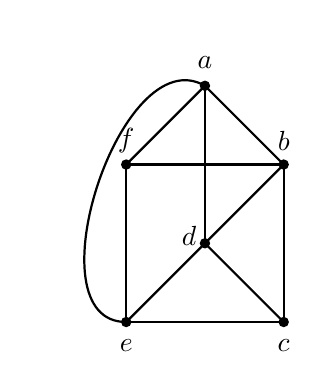
\begin{tikzpicture}
\coordinate (a) at (1,3);
\coordinate (b) at (2,2);
\coordinate (c) at (2,0);
\coordinate (d) at (1,1);
\coordinate (e) at (0,0);
\coordinate (f) at (0,2);
\begin{scope}[thick]
% draws vertices
\node[circle, fill=black,scale = 0.4] at (a){};
\node[circle, fill=black,scale = 0.4] at (b){};
\node[circle, fill=black,scale = 0.4] at (c){};
\node[circle, fill=black,scale = 0.4] at (d){};
\node[circle, fill=black,scale = 0.4] at (e){};
\node[circle, fill=black,scale = 0.4] at (f){};
% labels vertices
\node at (1,3.3) {$a$};
\node at (2,2.3) {$b$};
\node at (2,-0.3) {$c$};
\node at (0.8,1.1) {$d$};
\node at (0,-0.3) {$e$};
\node at (0,2.3) {$f$};
% draws edges
\draw[postaction={decorate}] (a) to (b);
\draw[postaction={decorate}] (b) to (c);
\draw[postaction={decorate}] (c) to (d);
\draw[postaction={decorate}] (d) to (e);
\draw[postaction={decorate}] (e) to (f);
\draw[postaction={decorate}] (c) to (e);
\draw[postaction={decorate}] (f) to (a);
\draw[postaction={decorate}] (f) to (b);
\draw[postaction={decorate}] (d) to (b);
\draw[postaction={decorate}] (a) to (d);
\draw[postaction={decorate},out=150,in=180] (a) to (e);
\end{scope}
\end{tikzpicture}
\end{center}
Solution:

It is cannot give a Euler Circuit, since the vertex $c$ and $f$ has degree of 3, which is not even, cannot satisfy the requirement of all even degree. The Euler path is 

\[c,b,d,c,e,a,d,e,f,b,a,f\]
\end{problem}
\begin{problem}{\S 10.5 - 26} For which values of $n$ do these graphs have an Euler
circuit?
\begin{enumerate}
\item[(a)] $K_n$
\item[(b)] $C_n$
\item[(c)] $W_n$
\item[(d)] $Q_n$
\end{enumerate}
Solution:
\begin{enumerate}
\item[(a)] $K_n$ Since all vertices are connected with each other, and there are total $n$ vertices, each vertices are connected to $n-1$ vertices, so, degree is $n-1$, so, to satisfy all have even degree, the $n$ should be odd.
\item[(b)] $C_n$ This forms a circle, which each vertices have exactly degree of 2 for $n\geq 3$, which automatically satisfies all vertices have even degree, so for every $n\geq 3$, it have an Euler circuit.
\item[(c)] $W_n$ This forms a wheel with a circle around a center, and since all vertices on the circle have degree of 3, it is all odd for every $n$, There is no Euler circuit for a wheel.
\item[(d)] $Q_n$ This is a cube in $n$ dimension, so each vertex are connected with $n$ vertices, so when $n$ is even but $n \neq 0$, it has Euler circuit.
\end{enumerate}
\end{problem}
\begin{problem}{\S 10.5 - 30} Determine whether the given graph has a
Hamilton circuit. If it does, find such a circuit. If it does not,
give an argument to show why no such circuit exists
\begin{center}
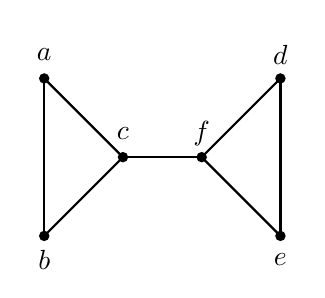
\begin{tikzpicture}
\coordinate (a) at (0,1);
\coordinate (b) at (0,-1);
\coordinate (c) at (1,0);
\coordinate (d) at (3,1);
\coordinate (e) at (3,-1);
\coordinate (f) at (2,0);
\begin{scope}[thick]
% draws vertices
\node[circle, fill=black,scale = 0.4] at (a){};
\node[circle, fill=black,scale = 0.4] at (b){};
\node[circle, fill=black,scale = 0.4] at (c){};
\node[circle, fill=black,scale = 0.4] at (d){};
\node[circle, fill=black,scale = 0.4] at (e){};
\node[circle, fill=black,scale = 0.4] at (f){};
% labels vertices
\node at (0,1.3) {$a$};
\node at (0,-1.3) {$b$};
\node at (1,0.3) {$c$};
\node at (3,1.3) {$d$};
\node at (3,-1.3) {$e$};
\node at (2,0.3) {$f$};
% draws edges
\draw[postaction={decorate}] (a) to (b);
\draw[postaction={decorate}] (b) to (c);
\draw[postaction={decorate}] (c) to (a);
\draw[postaction={decorate}] (d) to (e);
\draw[postaction={decorate}] (e) to (f);
\draw[postaction={decorate}] (f) to (d);
\draw[postaction={decorate}] (c) to (f);
\end{scope}
\end{tikzpicture}
\end{center}
Since edge $c-f$, it cannot form a simple circuit passing through all vertices in this graph.
\end{problem}
\end{document}